\documentclass{beamer} 
\usepackage{beamerthemeTUM}
\usepackage[latin1]{inputenc} 
\usepackage{amsmath} 
\usepackage{amsfonts} 
\usepackage{amssymb} 
\usepackage{algorithm} 
\usepackage{algorithmicx} 
\usepackage[noend]{algpseudocode}
\usepackage{multicol} 
\usepackage{url}
\usepackage{graphics}
\usepackage{multicol}
\usepackage{eso-pic}
\usepackage{pst-node}
\usepackage{xcolor}
\usepackage{multido}
\usepackage{subfigure}
\usepackage{pstricks}
\usepackage{float} 

\graphicspath{{figures/}}

\setlang{en}


\author{Sebastian Lehnerer} 
\title{Multilabel Attribute Selection} 

\subtitle{cluster based group selection}
\email{lehnerer@in.tum.de}
\date{\today}
\institute[2011]{Technische Universit\"at M\"unchen}


\begin{document} 


\AddToShipoutPicture{\TitlePicture}
\maketitle
%\frame{\titlepage}
\ClearShipoutPicture
\AddToShipoutPicture{\BackgroundPicture}
\AtBeginPart{\frame{\partpage}}

\frame{
 {\insertsection} 
 \begin{itemize} 
  \item using transposed dataset, each attribute will become an instance
  \item clustering over those instances
  \item clusters resolve directly into groups by splitting into labels and features
 \end{itemize}
}


\frame{
 {\insertsection} 
		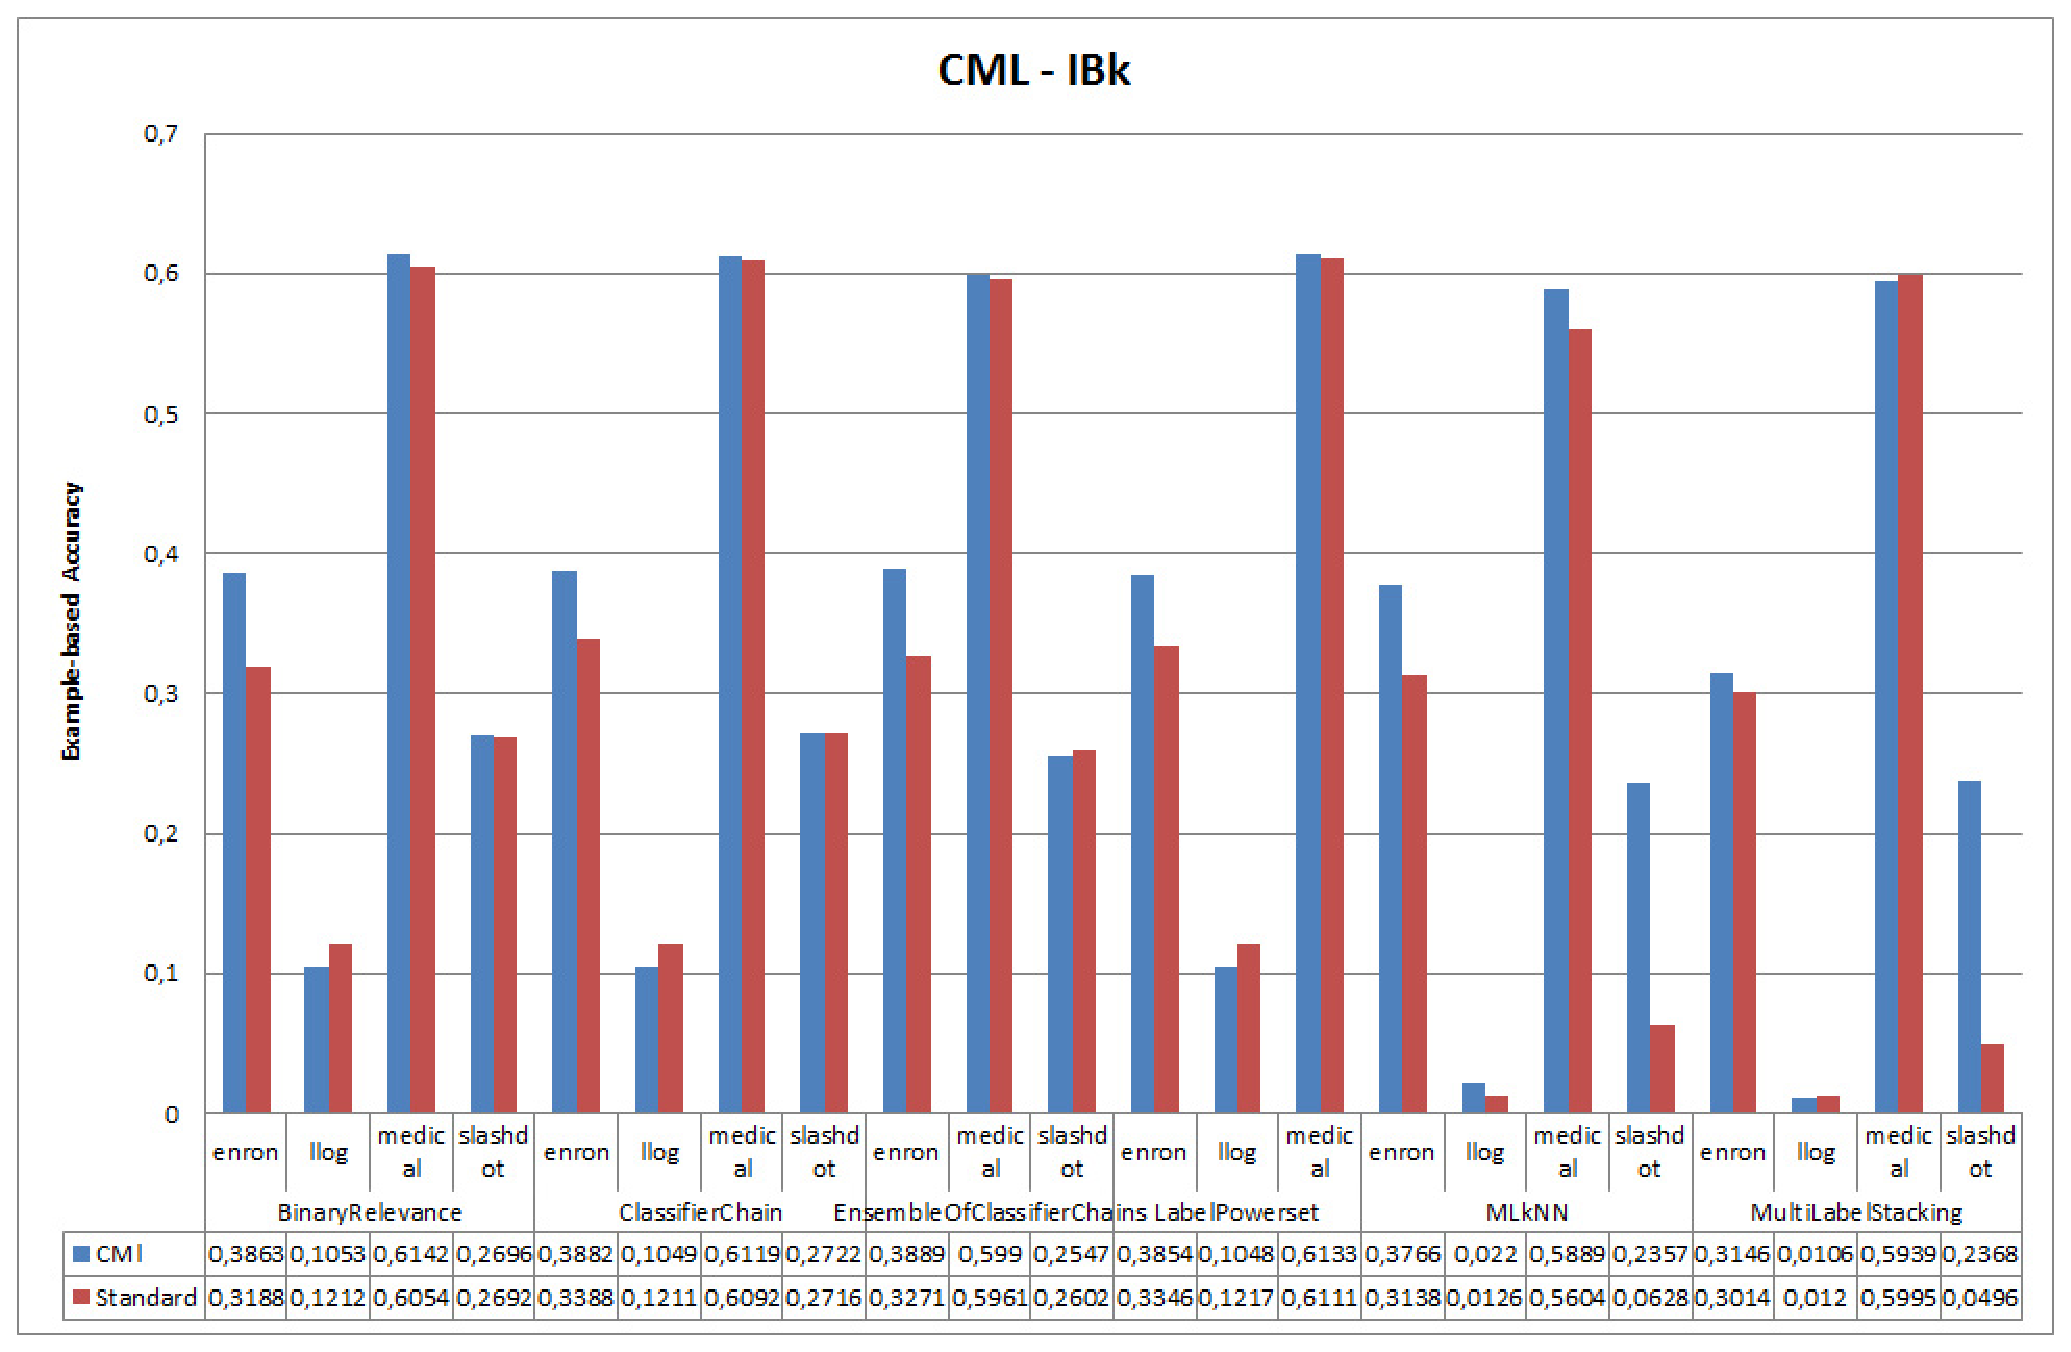
\includegraphics[scale=.3]{figures/cml_results_ibk.eps} 
}


\frame{
 {\insertsection} 
		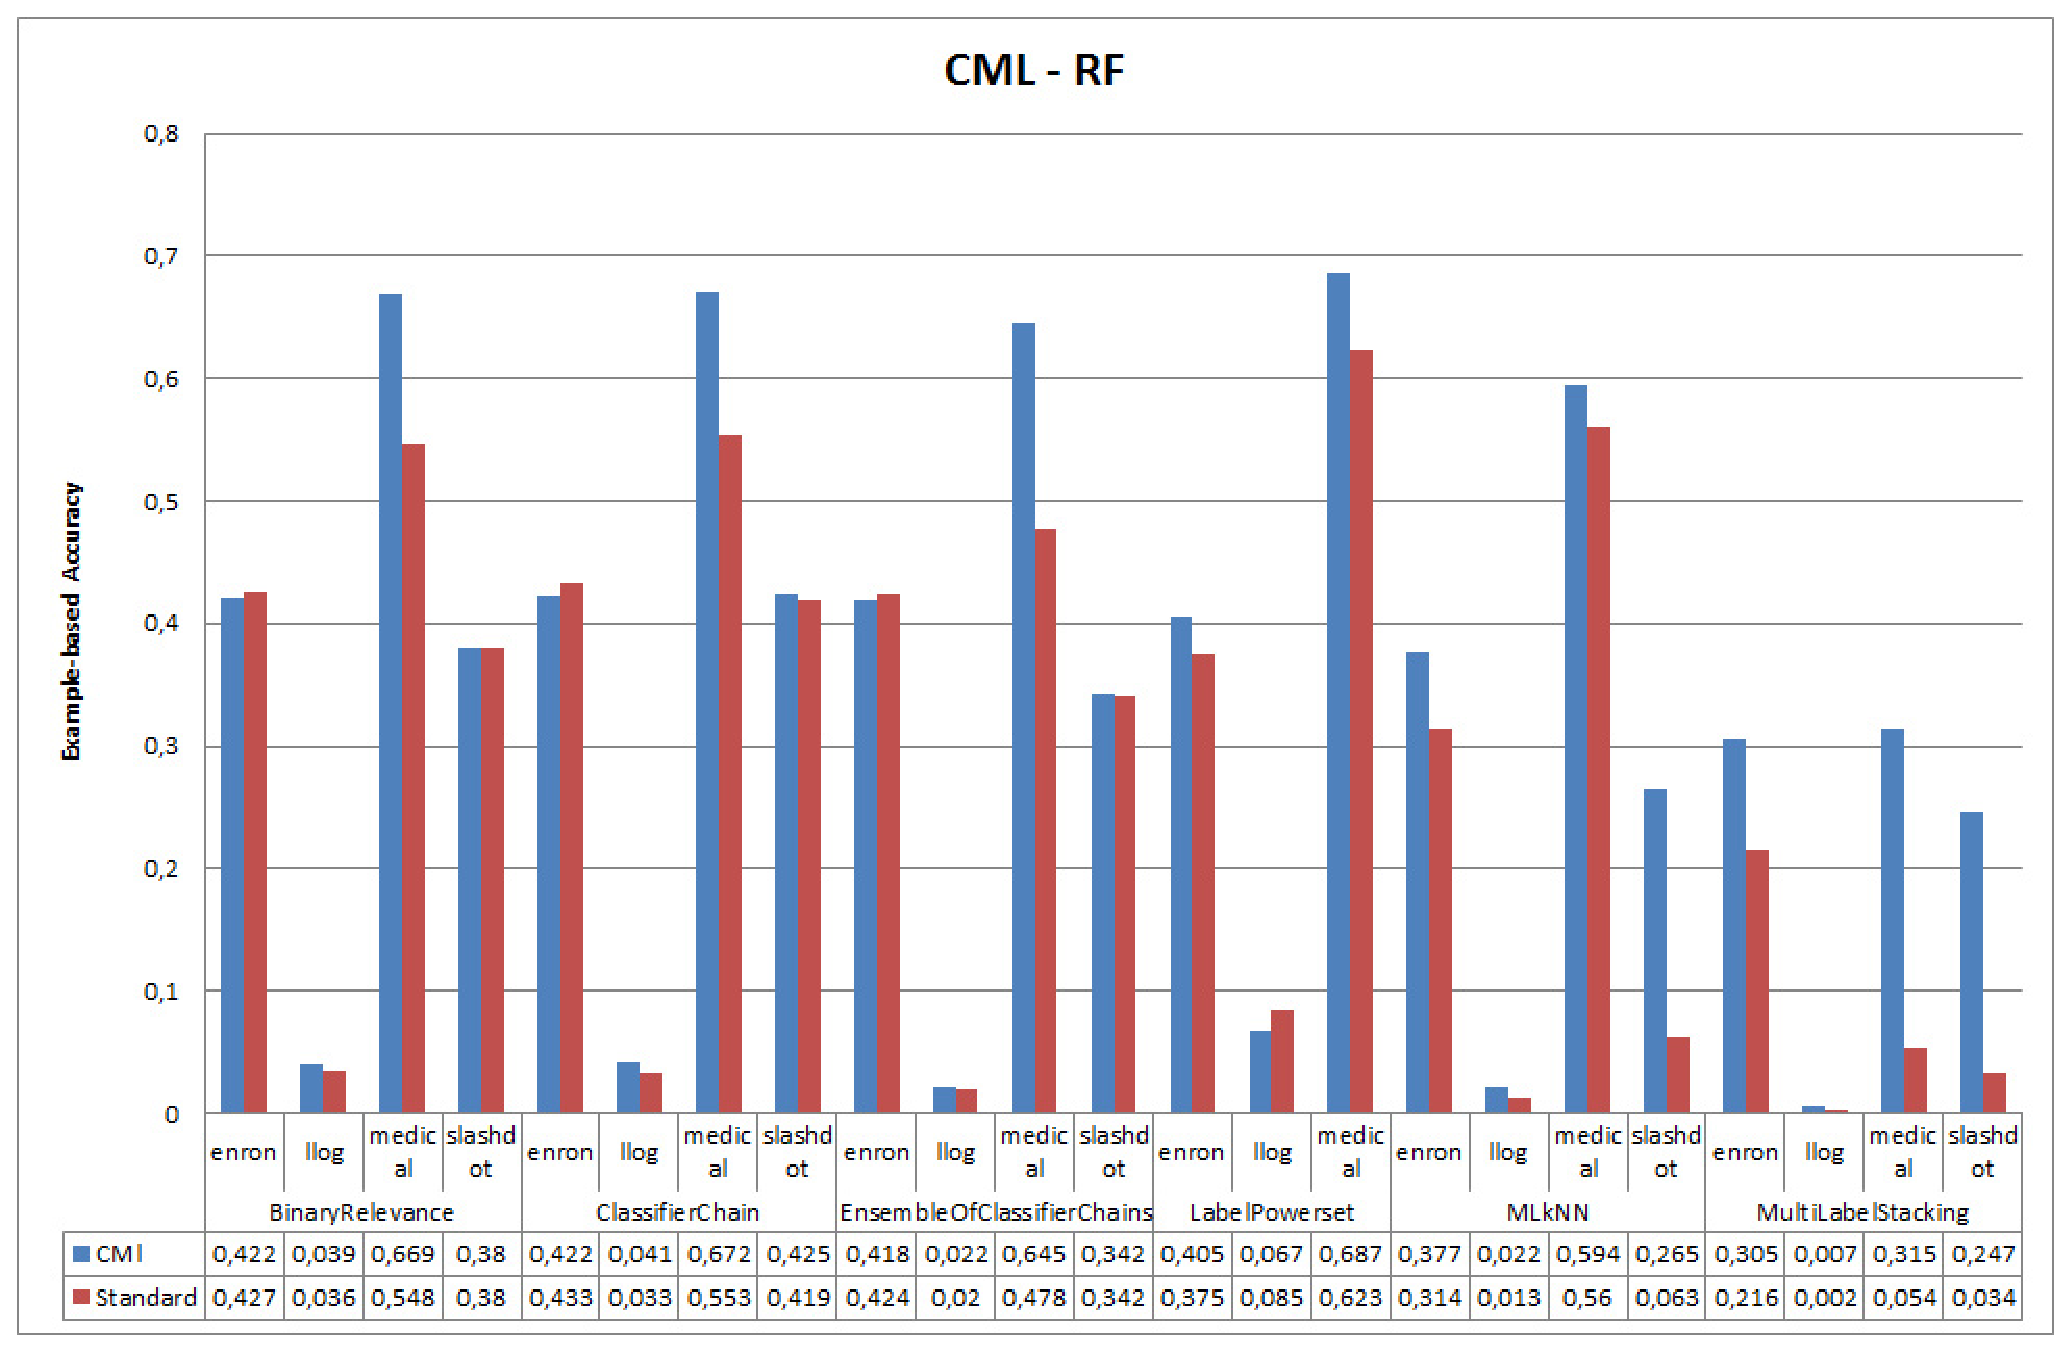
\includegraphics[scale=.3]{figures/cml_results_rf.eps} 
}


\frame{
 {\insertsection} 
		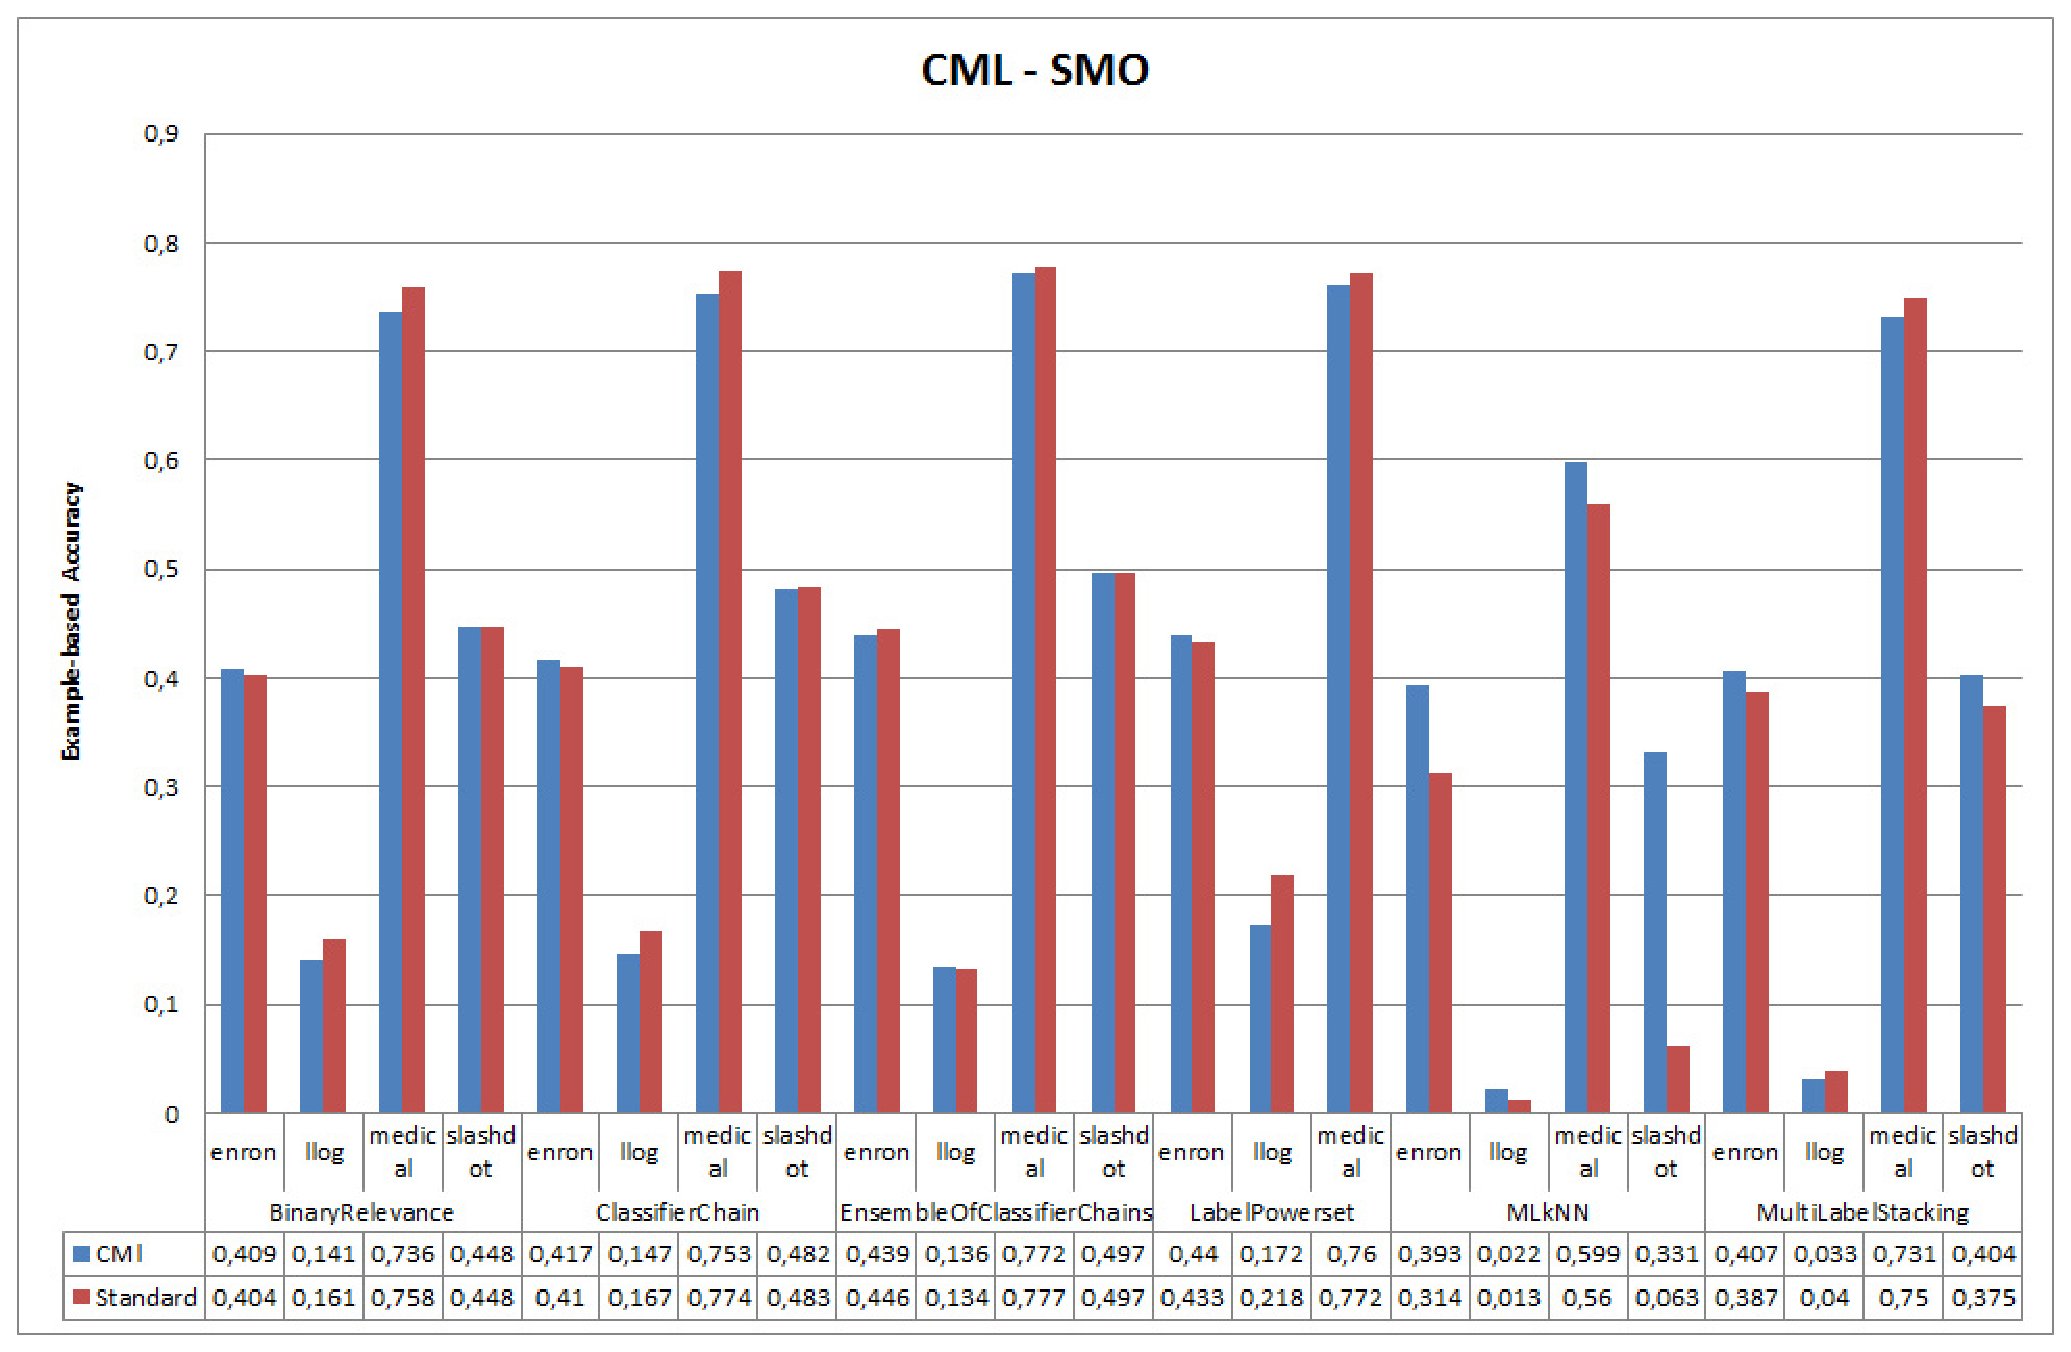
\includegraphics[scale=.3]{figures/cml_results_smo.eps} 
}

\frame{
	{\insertsection}
	example cluster characteristics (\(\varnothing\) over folds)
	\scriptsize {
	\begin{itemize}
		\item enron\\
		\(\varnothing\) number of clusters : 8\\
		\(\varnothing\) number of cluster ($> 2$ labels) : 2\\
		\(\varnothing\) number of labels per cluster: 13.3	
		\item llog\\
		\(\varnothing\) number of clusters : 4\\
		\(\varnothing\) number of cluster ($> 2$ labels) : 4\\
		\(\varnothing\) number of labels per cluster: 37.5	
		\item medical\\
		\(\varnothing\) number of clusters : 8.4\\
		\(\varnothing\) number of cluster ($> 2$ labels) : 2\\
		\(\varnothing\) number of labels per cluster: 10.7	
		\item slashdot\\
		\(\varnothing\) number of clusters : 10\\
		\(\varnothing\) number of cluster ($> 2$ labels) : 2\\
		\(\varnothing\) number of labels per cluster: 4.4	
	\end{itemize}
	}
}

\end{document}